\chapter{Cyclic Groups}

\section{Introduction}

For every positive integer $n$, we consider the integers modulo $n$. 

\begin{example}
    For $n = 3$, we have the multiplication table:

    \begin{minipage}[h]{0.45\linewidth} \begin{center}
        \begin{tabular}{c|c|c|c}
            $+$ & 0 & 1 & 2 \\ \hline
            0   & 0 & 1 & 2 \\ \hline
            1   & 1 & 2 & 0 \\ \hline
            2   & 2 & 0 & 1
        \end{tabular}
    \end{center} \end{minipage}
    \begin{minipage}[h]{0.45\linewidth} \begin{center}
        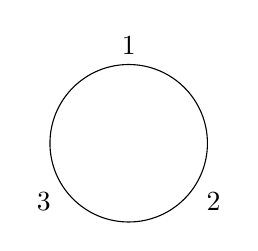
\begin{tikzpicture}
            \draw (0, 0) circle (1);
            
            \node[above] (1) at (0, 1) {1};
            \node[below right] (2) at (0.866, -0.5) {2};
            \node[below left] (3) at (-0.866, -0.5) {3};

            % Arc from 1 to 2, 2 to 3, 3 to 1, with text $+1$ on each arc
            % TODO
        \end{tikzpicture}
    \end{center} \end{minipage}

    Similarly, for $n = 4$, we have the multiplication table:

    \begin{table}[ht!]
        \centering
        \begin{tabular}{c|c|c|c|c}
            $+$ & 0 & 1 & 2 & 3 \\ \hline
            0   & 0 & 1 & 2 & 3 \\ \hline
            1   & 1 & 2 & 3 & 0 \\ \hline
            2   & 2 & 3 & 0 & 1 \\ \hline
            3   & 3 & 0 & 1 & 2
        \end{tabular}
    \end{table}
\end{example}

\begin{definition}[Cuclic Group]\index{Cyclic Group}\label{def:cyclic-group}
    A \term{cyclic group} is a group $G$ that has a generator. 
\end{definition}

\begin{definition}[Generator]\index{Generator}\label{def:generator}
    A \term{generator} of a group $G$ is an element $g \in G$ such that every element of $G$ can be written as a power of $g$.
\end{definition}

The group of integers modulo $n$ is called the \term{cyclic group of order $n$} and is denoted by $C_n$ or $\ZZ/n\ZZ$.

\begin{example}
    The integers $\ZZ$ form a cyclic group under addition. \[ 
        \cdots \xrightarrow{+1} -2 \xrightarrow{+1} -1 \xrightarrow{+1} 0 \xrightarrow{+1} 1 \xrightarrow{+1} 2 \xrightarrow{+1} \cdots 
    \]
\end{example}

Given a group $G$ and an element $g \in G$, we produce \[
    \underbrace{\left\{ \dots, g^{-2}, g^{-1}, 1 = g^0, g, g^2, g^3, \dots \right\}}_{\langle g \rangle} \subseteq G
\]

\begin{proposition}\label{prop:order-of-cyclic-group}
    Let $G$ be a group and $g \in G$. 

    \begin{listo}
        \item The set of powers of $g$, \[
            \left\{ g^m \mid m \in \ZZ \right\}
        \] is a subgroup of $G$ (denoted by $\langle g \rangle$).

        \item $g$ has order $m$ if and only if $\langle g \rangle$ is isomorphic to $C_m$.
        
        \item $g$ has no order if and only if $\langle g \rangle$ is isomorphic to $\ZZ$.
    \end{listo}
\end{proposition}

\begin{proof}(Proposition \ref{prop:order-of-cyclic-group}.1)
    WTS $\langle g \rangle$ is a subgroup of $G$.

    \begin{listu}
        \item \textbf{Associativity} follows from that of $G$. 

        \item \textbf{Identity} is a power of $g$, namely, $g^0 = 1$.

        \item Each element has an \textbf{inverse}, indeed, the inverse of $g^n$ is $g^{-n}$ which is also a power. 

        \item \textbf{Closed} under the operation \[
            g^n \cdot g^m = g^{n + m}
        \] which is also a power. 
    \end{listu}
\end{proof}

\begin{proof}(Proposition \ref{prop:order-of-cyclic-group}.2)
    WTS $g$ has order $m$ if and only if $\langle g \rangle \cong C_m$.

    If $G$ has order $m$, \[
        1, g, g^2, \dots, g^{m - 1}
    \] are distinct.

    Define $\Phi: C_m \to \langle g \rangle$ by $\Phi(k) = g^k$.

    This is well defined if $a \equiv b \pmod{m}$, then $a = b + mt$ for some $t \in \ZZ$. \[
        g^a = g^{b + mt} = g^b \cdot g^{mt} = g^b \cdot (g^m)^t = g^b \cdot 1^t = g^b
    \] 

    It is an homomorphism, indeed, \[
        \Phi(a + b) = g^{a + b} = g^a \cdot g^b = \Phi(a) \cdot \Phi(b)
    \]

    \begin{listu}
        \item \textbf{Injectivity}
        
        If $\Phi(a) = \Phi(b)$, then $g^a = g^b$, so $g^{a - b} = 1$.

        We can pick $a, b \in \{ 0, 1, \dots, m - 1 \}$. We can also suppose $a \ge b$, thus \[
            0 \le a - b \le m - 1
        \]

        Then $g^{a - b} = 1$ implies $a - b = 0$, for owtherwise $g$ has order smaller than $m$. 

        Thus, $a = b$, so $\Phi$ is injective.

        \item \textbf{Surjectivity}

        By assumption \[
            \langle h \rangle = \{ g^0, g^1, \dots, g^{m - 1} \}
        \]

        Since by definition \[
            \Phi(k) = g^k,
        \] by taking $k = 0, 1, \dots, m - 1$ we produce all elements of $\langle g \rangle$.

        Thus, $\Phi$ is surjective.
    \end{listu}

    We conclude that $\Phi$ is an isomorphism.
\end{proof}

\begin{example}
    Consider $C_6 = \{ 0, 1, 2, 3, 4, 5 \}$.

    The cyclic groups the elements generate are
    \begin{listu}
        \item $0$ generates $\{ 0 \} \equiv C_1$.
        \item $1$ and $5$ generate $\equiv C_6$, $C_6 = \langle 1 \rangle = \langle 5 \rangle$.
        \item $\langle 2 \rangle = \{ 0, 2, 4\} = \langle 4 \rangle \cong C_3$. 
        \item $\langle 3 \rangle = \{ 0, 3 \} \cong C_2$.
    \end{listu}
\end{example}

\begin{example}
    We have already seen in a previous example what happens. The cyclic subgroups are

    \begin{listu}
        \item $\langle 1 \rangle = \{ \id \} = C_1$.
        \item $\langle (1, 2) \rangle = \{ \id, \langle (1, 2) \rangle \} = C_2$
        \item $\langle (1, 3) \rangle = \{ \id, \langle (1, 3) \rangle \} = C_2$
        \item $\langle (2, 3) \rangle = \{ \id, \langle (2, 3) \rangle \} = C_2$
        \item $\langle (1, 2, 3) \rangle = \{ \id, (1, 2, 3), (1, 3, 2) \rangle \} = C_3$
    \end{listu}
\end{example}

\begin{proposition}
    Let $p$ be a prime number. The only group of order $p$ is $C_p$. 
\end{proposition}

\begin{proof}
    {~~~}

    Let $G$ be a group of order $p$. Since $p$ is prime, $G$ has at least two elements. Thus, there exists $g \in G$ with $g \neq e$. 

    % TODO
\end{proof}